\providecommand{\main}{..}
\documentclass[dvipdfmx]{jsarticle}
\usepackage[dvipdfmx]{graphicx}

\usepackage{ascmac}
\usepackage{lib_ulinej}
\usepackage{lib_bendarrow}
\usepackage{amsmath}
\usepackage{datetime}
\usepackage{comment}
\usepackage{framed}
\usepackage{arydshln}
\usepackage{breqn}
\usepackage{graphicx}
\graphicspath{{\main/imgs/}{imgs/}}

%https://stackoverflow.com/questions/722613/centering-a-table-wider-than-the-text-column
\usepackage{chngpage} % allows for temporary adjustment of side margins

%スクリプトの記述用
\usepackage{color}
\usepackage{listings,lib_jlisting}

%適切な場所に画像等を表示
\usepackage{here}

%listoftables用
\usepackage{tocloft}

%余白
\usepackage[top=4cm, bottom=3cm, left=2cm, right=2cm]{geometry}

%bibtex用
\usepackage{url}
\usepackage{natbib}
\setcitestyle{aysep={}}  %著者名と年の間にカンマを入れない

%platex文字化け対策
\usepackage[utf8]{inputenc}

%タイトルのスペース
\usepackage{titlesec}

%表のキャプションをサイト
\usepackage[hidelinks,colorlinks=false]{hyperref}
\usepackage{lib_pxjahyper}%日本語の文字化け防止

%ページずれ防止


%言語の設定
\lstset{%
  tabsize=4, % Tabを何文字幅にするかの指定
%  language={R}, % 言語の指定
  basicstyle={\ttfamily\small}, % 標準の書体の指定
  backgroundcolor={\color[gray]{.90}},%背景色
%  identifierstyle={¥scriptsize}, % キーワードでない文字の書体
%  commentstyle={¥scriptsize¥itshape},% コメントの書体
%  keywordstyle={¥scriptsize¥bfseries},% キーワードの書体
%  ndkeywordstyle={¥scriptsize},% キーワードの書体その2
%  stringstyle={¥scriptsize¥ttfamily}, % ""で囲まれた文字の書体
  columns=[l]{fullflexible},% 書体による列幅の違いを調整するか
%  frame={tbl}, %枠追加
%  frameround=ftff,%フレーム角の形状
  framesep=5pt,%本文からframeまでの間隔
  breaklines=true, % 行が長くなった場合の改行
  numbers=left, % 左側に行番号追加
  xrightmargin=0zw,%
  xleftmargin=1zw,%
  numberstyle={\scriptsize},% 行番号のスタイル
  stepnumber=1, % 行番号をいくつ飛ばしで表示するか
%  numbersep=1zw,% 行番号と本文の間隔。デフォルトは10pt
  lineskip=-0.5ex, % 行間の調整
  showstringspaces=false
}

\title{\vspace{-3cm} タイトル} 
\author{\vspace{-1cm} 筆者名\thanks{所属とメアド}}
\date{最終更新:~\today~\currenttime~(JST)}

\begin{document}

    \maketitle

    \setcounter{tocdepth}{3}
    % 3 = \subsubsectionまで
    \tableofcontents

    \makeatletter
    \renewcommand\listoftables{%
        \@starttoc{lot}%
    }

    \section*{概要}
        2017年に収集されたほにゃらららら\citep{nikkeidram4takai}\citep{akibagpu}
        \begin{eqnarray}
            \left( \frac{\partial x}{\partial n}\right) &=& aaaaaaaaaa\label{siki1}\\
            2 &=& 1 \cdot 2
        \end{eqnarray}
    \section{導入}
        \begin{lstlisting}
            //ここにコードを書く
            $php = hoge(aaaaaa);
        \end{lstlisting}

    \newpage
    \phantomsection
        
    \section*{付録}
      \addcontentsline{toc}{section}{付録} 
      %https://githubtycom/akira-okumura/MasterThesisTemplate/blob/master/Appendixtytex
      \setcounter{subsection}{0} % section の番号をゼロにリセットする
      \renewcommand{\thesubsection}{\Alph{subsection}} % 数字ではなくアルファベットで数える
      \setcounter{subsubsection}{0} % 式番号を Aty1 のようにする
      \renewcommand{\thesubsubsection}{\Alph{subsection}.\arabic{subsubsection}}
      \setcounter{equation}{0} % 式番号を Aty1 のようにする
      \renewcommand{\theequation}{\Alph{subsection}.\arabic{equation}}
      \setcounter{figure}{0} % 図番号
      \renewcommand{\thefigure}{\Alph{subsection}.\arabic{figure}}
      \setcounter{table}{0} % 表番号
      \renewcommand{\thetable}{\Alph{subsection}.\arabic{table}}

    
      \subsection{図}
        \subsubsection{ヒートマップ(すべての契約期間のデータ)}
          \label{heatmap_all}
          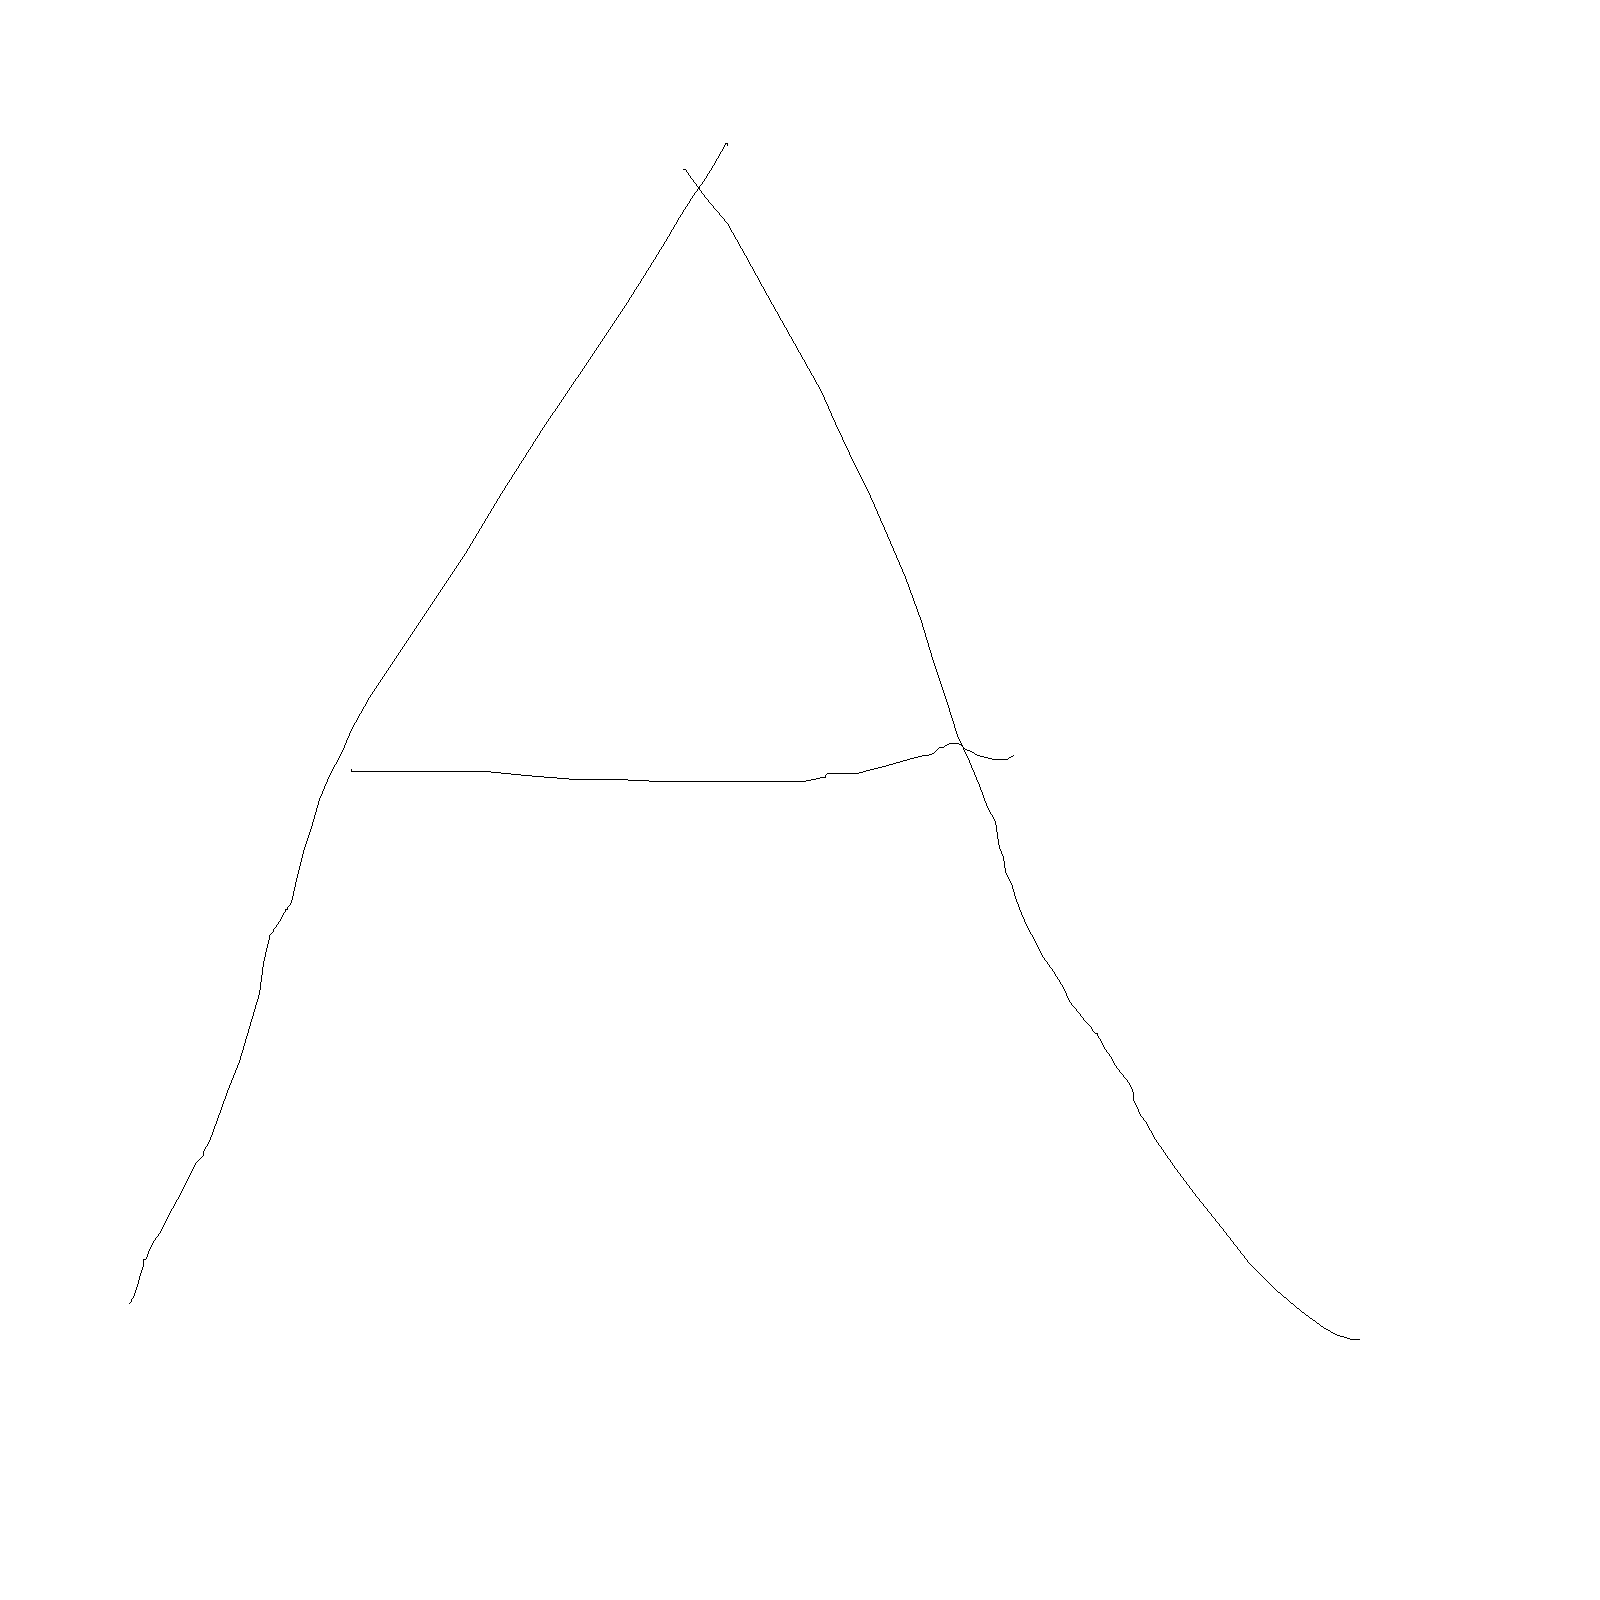
\includegraphics[width=20cm]{figure_heatmap_all.png}\\

      \clearpage

      \subsection{表}

        \subsubsection{  \nameref{hyob_spec1_reset} }
          \begin{table}[!htbp] \centering 
            \caption{式(\ref{siki1})のRamsey RESET検定の結果} 
            \label{hyob_spec1_reset} 
              \begin{tabular}{lll}
                %1つめの定式化の回帰 
                Title                          &       Ramsey RESET test \\
                F-value                        &         aaaaa \\
                p-value                        &  aaaaaa \\
                Numerator degree of freedom    &                     aaaa \\
                Denominator degrees of freedom &                   aaa \\
                \end{tabular}
          \end{table} 
        
       \clearpage
        %%%%%%%%%%%%%%%%%%%%%%%%%%%%%%%%%%%%%%%%%%%%
        %        記述統計量          %
        %%%%%%%%%%%%%%%%%%%%%%%%%%%%%%%%%%%%%%%%%%%%
        \subsubsection{  \nameref{hyob_1} }
          \vspace{-0.5cm}
          \begin{table}[!htbp] \centering 
            \caption{記述統計表} 
            \label{hyob_1} 
            \begin{adjustwidth}{-1in}{-1in} \begin{center} \resizebox{1.0\textwidth}{!}{ %サイズ調整開始       
              \begin{tabular}{lrrrrrrrrrrrrrrrrrrrrrrrr}
                {} &  contract\_length &  aaaaa &       is\_3G &  promo\_data\_GB &  bbbb &  aaaaa \\
                count &      aaaaaa &  sddddtyvcxcdf00 &  sddddtyvcxcdf00 &     137tyvcxcdf00 &           sddddtyvcxcdf00 &    sddddtyvcxcdf0 \\
                mean  &         7ty865065 &    0ty05360vcxcdf &    0ty011091 &      10ty928vcxcdf67 &            aaaaa &   5190ty82589 \\
                std   &         9ty393570 &    0ty225vcxcdfvcxcdfvcxcdf &    0ty10vcxcdf823 &      20ty27vcxcdf031 &             2ty982298 &  22170ty12797 \\
                min   &         1tyvcxcdf00 &    0tyvcxcdf00 &    0tyvcxcdf00 &       0tyvcxcdf00 &             0tyvcxcdf00 &      0ty02000 \\
                25\%   &         1tyvcxcdf00 &    0tyvcxcdf00 &    0tyvcxcdf00 &       0tyvcxcdf00 &             0tyvcxcdf00 &      3tyvcxcdf0 \\
                50\%   &         1tyvcxcdf00 &    0tyvcxcdf00 &    0tyvcxcdf00 &       3tyvcxcdf00 &             0tyvcxcdf00 &      8tyvcxcdf0 \\
                75\%   &        12tyvcxcdf00 &    0tyvcxcdf00 &    0tyvcxcdf00 &      10tyvcxcdf00 &             0tyvcxcdf00 &     20tyvcxcdf0 \\
                max   &        2vcxcdftyvcxcdf00 &    1tyvcxcdf00 &    1tyvcxcdf00 &     110tyvcxcdf00 &            2vcxcdftyvcxcdf00 &  99999tyvcxcdf0 \\  
              \end{tabular}
            } \end{center} \end{adjustwidth} %サイズ調整終わり
            \begin{adjustwidth}{-1in}{-1in} \begin{center} \resizebox{1.0\textwidth}{!}{ %サイズ調整開始       
              \begin{tabular}{lrrrrrrrrrrrrrrrrrrrrrrrr}
                \\
                {} &  data\_average\_GB &   promo\_1\_JPY &  promo\_1\_dur &  non\_promo\_JPY &  access\_fee\_JPY &  rebate\_monthly\_JPY \\
                count &       sddddtyvcxcdf00 &    sddddtyvcxcdf00 &   sddddtyvcxcdf00 &     sddddtyvcxcdf00 &      sddddtyvcxcdf00 &          sddddtyvcxcdf00 \\
                mean  &      xxxxx91ty111272 &    293ty8766vcxcdf7 &     0ty756007 &    6128ty13520vcxcdf &       xxxxxx &           vcxcdf7tysdddd1209 \\
                std   &     22170ty06128vcxcdf &   1157ty657990 &     3ty253998 &    380vcxcdfty719222 &      vcxcdf01ty768621 &          2vcxcdf5ty667897 \\
                min   &         0ty02sdddd &      0tyvcxcdf00 &     0tyvcxcdf00 &     307tyvcxcdf29000 &        0tyvcxcdf00 &            0tyvcxcdf00 \\
                25\%   &         3ty333330 &      0tyvcxcdf00 &     0tyvcxcdf00 &    3vcxcdf79ty996700 &        0tyvcxcdf00 &            0tyvcxcdf00 \\
                50\%   &         8ty75vcxcdf &      0tyvcxcdf00 &     0tyvcxcdf00 &    518vcxcdfty308vcxcdf21 &        0tyvcxcdf00 &            0tyvcxcdf00 \\
                75\%   &        20tyvcxcdf00 &      0tyvcxcdf00 &     0tyvcxcdf00 &    7928ty907127 &        0tyvcxcdf00 &            0tyvcxcdf00 \\
                max   &     99999tyvcxcdf00 &  10560ty007500 &    2vcxcdftyvcxcdf00 &   31037ty33vcxcdf59vcxcdf &     2vcxcdf85tyvcxcdf00 &         2682ty75vcxcdf \\
              \end{tabular}
                } \end{center} \end{adjustwidth} %サイズ調整終わり
            \end{table} 

    \newpage
    \phantomsection
    \section*{参考文献}
    \addcontentsline{toc}{section}{参考文献} 
    \bibliographystyle{jecon}
    %タイトルを消す
    \renewcommand{\bibsection}{}
    \bibliography{kncitations}


\end{document}



%下 記述例
%\begin{itembox}[c]{ヒントと注意}
%   まずは UMP を解かないと話が始まりません。
%\end{itembox}
%
%  \includegraphics[width=16cm]{toi42.png}
%
%\text{rtarrow}\rtarrow,\text{rbarrow}\rbarrow,\text{ltarrow}\ltarrow,\text{lbarrow}\lbarrow \\\\
%
%   \begin{enumerate}
%    \setlength{\leftskip}{2.5mm}
%    \renewcommand{\labelenumi}{Step \theenumi.}
%    \item A
%    \item B
%   \end{enumerate}
%
%   \begin{screen}
%       (a)~(c)
%       \begin{enumerate}
%           \renewcommand{\labelenumi}{(\alph{enumi})}
%           \item A
%           \item B
%       \end{enumerate}
%   \end{screen}
%
%\begin{shadebox}
%    ①~
%    \begin{enumerate}
%        \renewcommand{\labelenumi}{\textcircled{\scriptsize \theenumi}}
%        \item プレーヤーはAとBの2人
%        \item 同時に意志決定
%    \end{enumerate}
%\end{shadebox}
%
%\begin{table}[h]
%      \begin{center}
%        \begin{tabular}{|c|c|c|c|} \hline
%            A\B&グー&チョキ&パー \\  \hline
%            グー&0, 0&3, 0&0, 6 \\ \hline
%        \end{tabular}
%      \end{center}
%      \caption{(1)}
%      \label{(1)}
%\end{table}
%
%\begin{eqnarray*}
%    m &=& \frac{5}{21} \\
%    n &=& \frac{10}{21}
%\end{eqnarray*}
%
%増減表をつくる(必要な部分だけ埋めた)。
%\begin{table}[htb]
%  \centering
%  \begin{tabular}{c||c|c|c|c|c|c|c|c|c}
%    $x$               & 0    &          & &     & 10 \\ \hline
%    $u'$              &  &       &           & &    \\
%    $u^{\prime\prime}$&  &       &        &  & \\ \hline
%    $u$               &  &  & $\mbox{極大値}\atop    $ &   &  
%  \end{tabular}
%\end{table}
